\documentclass{standalone}
\usepackage{placeins}
\begin{document}


    \section{Design}
    Sparkling Water is designed to be executed as a regular Spark application. It provides a way to initialize H2O
    services on top of Spark and access data stored in data structures of Spark and H2O.

    Sparkling Water supports two type of backends - internal and external. In the internal backend, Sparkling Water starts
    H2O in Spark executors, which are created after application submission. At this point, H2O starts services,
    including distributed key-value (K/V) store and memory manager, and orchestrates the nodes into a cloud.
    The topology of the created cloud tries to match the topology of the underlying Spark cluster.
    The following figure represents the Internal Sparkling Water cluster.


    \begin{figure}[h!]
        \centering
        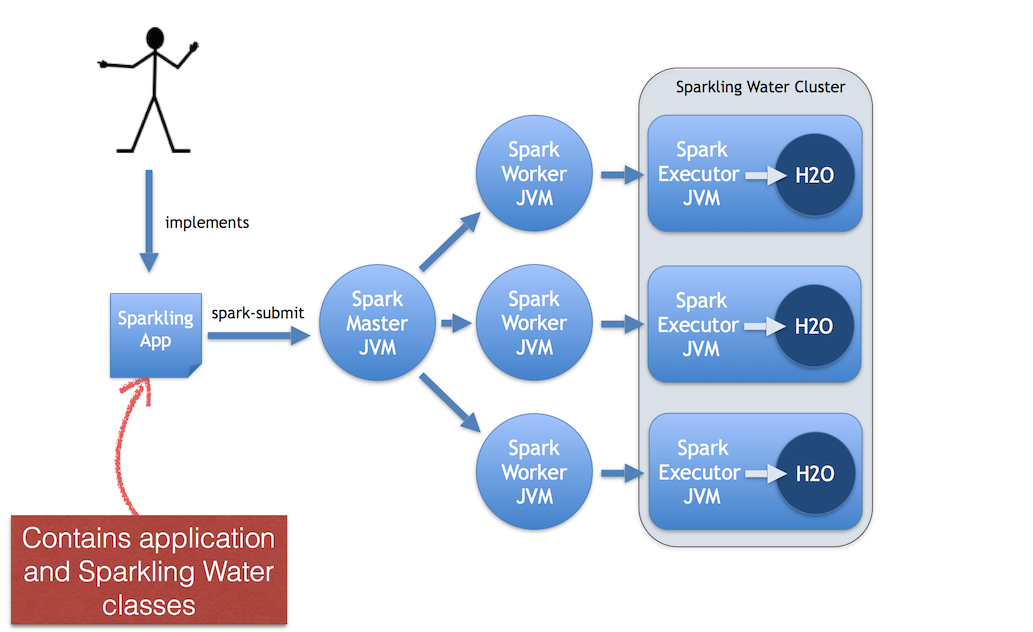
\includegraphics[scale=0.6]{../images/Topology-internal.png}
        \caption{Sparkling Water design depicting deployment of the Sparkling Water in internal backend to the Spark cluster.}
    \end{figure}

    In external backend, the H2O cluster is started separately and is connected to from the Spark driver. The
    following figure represents the External Sparkling Water cluster.

    \begin{figure}[h!]
        \centering
        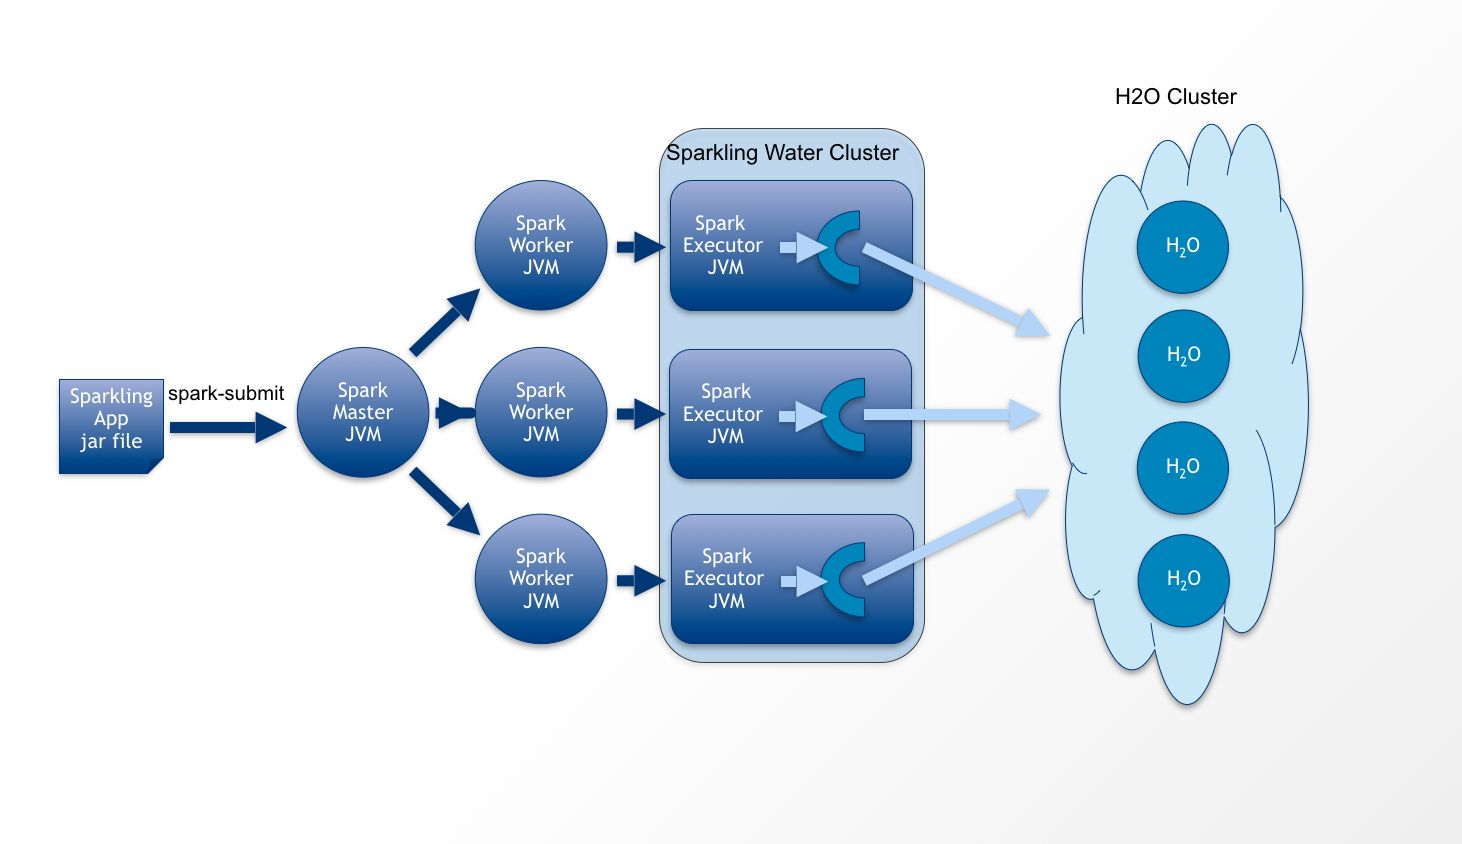
\includegraphics[scale=0.4]{../images/Topology-external.png}
        \caption{Sparkling Water design depicting deployment of the Sparkling Water in internal backend to the standalone Spark cluster.}
    \end{figure}

    More information about the backends and how to start Sparkling Water in each backend is available in the next section.

    \subsection{Data Sharing between Spark and H2O}

    Sparkling Water enables transformation between Spark data structures (RDD, DataFrame, Dataset) and H2O's
    \texttt{H2OFrame}, and vice versa.

    When converting a \texttt{H2OFrame} to a RDD or DataFrame, a wrapper is created around the \texttt{H2OFrame} to provide
    an RDD or DataFrame like API. In this case, data is not duplicated but served directly from the underlying \texttt{H2OFrame}.

    Converting from an RDD/DataFrame to an \texttt{H2OFrame} requires data duplication because it transfers
    data from the RDD storage into a \texttt{H2OFrame}. However, data stored in a \texttt{H2OFrame} is heavily compressed
    and does not need to be preserved in RDD after the conversion.

    The following figure shows how data is accessed when running in internal backend mode of Sparkling Water.

    \begin{figure}[h!]
        \centering
        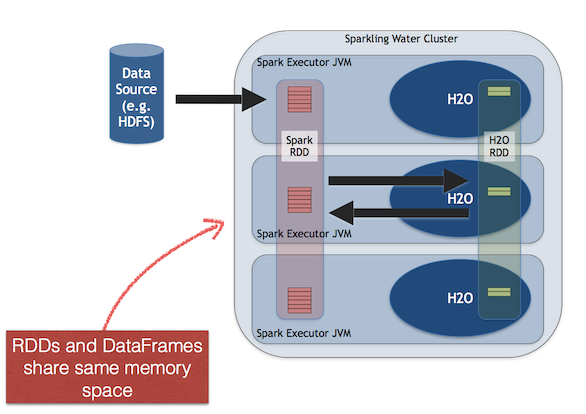
\includegraphics[scale=1]{../images/DataShare.png}
        \caption{Sharing between Spark and H2O inside an executor JVM in Internal backend.}
    \end{figure}

    In the external backend, the Spark and H2O data spaces are separated, however the separation is transparent to the user.

    \subsection{H2OContext}

    The main Sparkling Water component is \texttt{H2O Context}.
    H2O Context holds state and provides primitives to transfer RDD/DataFrames/Datasets into H2OFrames and vice versa.
    It follows design principles of Spark primitives such as \texttt{SparkSession}, \texttt{SparkContext} and \texttt{SQLContext}.


    \texttt{H2OContext} contains the necessary information for running H2O services and exposes methods for data
    transformation between the Spark RDD, \texttt{DataFrame} or \texttt{Dataset}, and the \texttt{H2OFrame}.
    Starting \texttt{H2OContext} involves an operation that:

    \begin{itemize}
        \item In case of internal backend, is distributed and contacts all accessible Spark executor nodes and initializes H2O services (such as the key-value store and RPC) inside the executors' JVMs.
        \item In case of external backend, either starts H2O cluster on YARN and connects to it or connects to existing H2O cluster right away (depends on the configuration).
    \end{itemize}

    The next sections show how to start H2OContext in all supported clients and both backends.
\end{document}
